\def\duedate{\today}
\def\HWnum{5}
\documentclass[10pt,a4paper]{book}

% custom section formatting
\usepackage{titlesec}
\titleformat{\chapter}[display]
{\normalfont\Large\filcenter\sffamily}
{\titlerule[1pt]%
\vspace{1pt}%
\titlerule
\vspace{1pc}%
\LARGE\MakeUppercase{\chaptertitlename} \thechapter}
{1pc}
{\titlerule
\vspace{1pc}%
\Huge}

% appendix handling
\usepackage[toc,page]{appendix}
    
% encoding for file and font
\usepackage[utf8]{inputenc}
\usepackage[T1]{fontenc}

% math formatting/tools
\usepackage{amsmath}
\usepackage{amssymb}
\usepackage{mathtools}
\usepackage[arrowdel]{physics}
\usepackage{dsfont}

\newcommand{\R}{\mathbb{R}}
\newcommand{\Z}{\mathbb{Z}}
\newcommand{\N}{\mathbb{N}}
\newcommand{\Q}{\mathbb{Q}}
\newcommand{\C}{\mathbb{C}}

% unit formatting
\usepackage{siunitx}
\AtBeginDocument{\RenewCommandCopy\qty\SI}

% figure formatting/tools
\usepackage{graphicx}
\usepackage{float}
\usepackage{subcaption}
\usepackage{multirow}
\usepackage{import}
\usepackage{pdfpages}
\usepackage{transparent}
\usepackage{currfile}

\NewDocumentCommand\incfig{O{1} m}{
    \def\svgwidth{#1\textwidth}
    \import{./Figures/\currfiledir}{#2.pdf_tex}
}

\newcommand{\bef}{\begin{figure}[h!tb]\centering}
\newcommand{\eef}{\end{figure}}

\newcommand{\bet}{\begin{table}[h!tb]\centering}
\newcommand{\eet}{\end{table}}

% hyperlink references 
\usepackage{hyperref}
\hypersetup{
    colorlinks=true,
    linkcolor=blue,
    filecolor=magenta,
    urlcolor=cyan,
    pdftitle={Physics 1 Notes},
    pdfauthor={Richard Whitehill},
    pdfpagemode=FullScreen
}
\urlstyle{same}

\newcommand{\eref}[1]{Eq.~(\ref{eq:#1})}
\newcommand{\erefs}[2]{Eqs.~(\ref{eq:#1})--(\ref{eq:#2})}

\newcommand{\fref}[1]{Fig.~(\ref{fig:#1})}
\newcommand{\frefs}[2]{Fig.~(\ref{fig:#1})--(\ref{fig:#2})}

\newcommand{\aref}[1]{Appendix~(\ref{app:#1})}
\newcommand{\sref}[1]{Section~(\ref{sec:#1})}
\newcommand{\srefs}[2]{Sections~(\ref{sec:#1})-(\ref{sec:#2})}

\newcommand{\tref}[1]{Table~(\ref{tab:#1})}
\newcommand{\trefs}[2]{Table~(\ref{tab:#1})--(\ref{tab:#2})}

% tcolorbox formatting/definitions
\usepackage[most]{tcolorbox}
\usepackage{xcolor}
\usepackage{xifthen}
\usepackage{parskip}

\definecolor{peach}{rgb}{1.0,0.8,0.64}

\DeclareTColorBox[auto counter, number within=chapter]{defbox}{O{}}{
    enhanced,
    boxrule=0pt,
    frame hidden,
    borderline west={4pt}{0pt}{green!50!black},
    colback=green!5,
    before upper=\textbf{Definition \thetcbcounter \ifthenelse{\isempty{#1}}{}{: #1} \\ },
    sharp corners
}

\newcommand*{\eqbox}{\tcboxmath[
    enhanced,
    colback=black!10!white,
    colframe=black,
    sharp corners,
    size=fbox,
    boxsep=8pt,
    boxrule=1pt
]}

\newtcolorbox[auto counter, number within=chapter]{exbox}{
    parbox=false,
    breakable,
    enhanced,
    sharp corners,
    boxrule=1pt,
    colback=white,
    colframe=black,
    before upper= \textbf{Example \thetcbcounter:}\,,
    before lower= \textbf{Solution:}\,,
    segmentation hidden
}

\newtcolorbox{resbox}{
    enhanced,
    colback=black!10!white,
    colframe=black,
    boxrule=1pt,
    boxsep=0pt,
    top=2pt,
    ams nodisplayskip,
    sharp corners
}


\begin{document}

\prob{1}{

Find the branch points of this function:
\begin{eqnarray}
   f(z) = \sqrt{z^2 + 2z - 1}
.\end{eqnarray}
What branch cuts can make this function single-valued?

}

\sol{

We can write
\begin{eqnarray}
    f(z) = \sqrt{\Big[z - \Big(-1 + \sqrt{2} \Big)\Big] \Big[z - \Big(-1 - \sqrt{2} \Big) \Big]}
.\end{eqnarray}
Thus, there are branch points at $z = -1 \pm \sqrt{2}$.
We can make a couple different branch cuts to make this function single valued such as those shown in \fref{prob1}.
The first is just connecting the two points via a line on the real axis, and the second is the lines $(\infty,-1 - \sqrt{2}]$ and $[-1 + \sqrt{2},\infty)$.

\begin{figure}[h!]
    \centering
    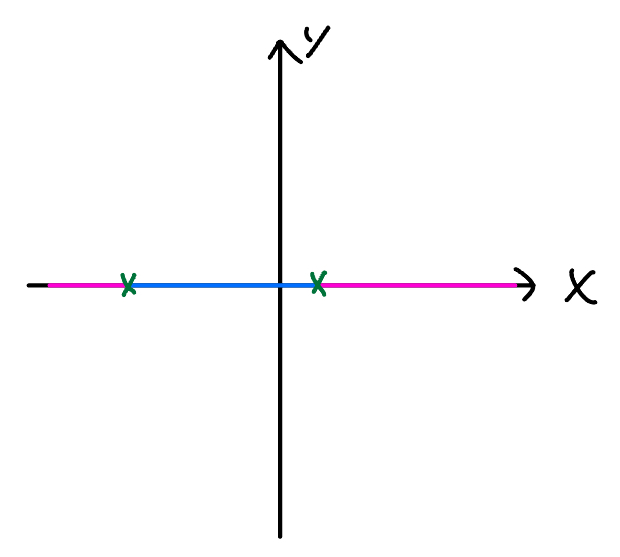
\includegraphics[width=0.4\textwidth]{prob1.jpeg}
    \caption{Sketch of branch points of the function $f(z) = \sqrt{z^2 + 2z - 1}$ and some possible branch cuts to make the function single valued. The blue line connects the two points, and the magenta lines extend from the points either to $\pm \infty$, depending on the sign of the branch point.}
    \label{fig:prob1}
\end{figure}

}


\prob{2}{

Find the residues and all isolated singularities of the function
\begin{eqnarray}
    I_{2}(z) = \tan{z}
.\end{eqnarray}

}

\sol{

Observe that
\begin{eqnarray}
    \tan{z} = \frac{\sin{z}}{\cos{z}} = \dfrac{\sin{z}}{\prod_{n=0}^{\infty} \Big[ 1 - \frac{4 z^2}{\pi^2(2n+1)^2} \Big]}
.\end{eqnarray}
Clearly, the function becomes singular at $z = \pm(n + 1/2)\pi$ for $n = 0,1,2,\ldots$, and furthermore, observe that these are all isolated singularities and simple poles.
Notice that in the neighborhood of these poles (let $z_{n} = (n + 1/2)\pi$ where $n = 0,\pm 1,\pm 2,\ldots$) we can write
\begin{eqnarray}
    \begin{aligned}
        \cos{z} &= \cos{(w + z_{n})} = \cos{w}\cos{z_{n}} - \sin{w} \sin{z_{n}} = (-1)^{n+1} \sin{w} \\
                &= (-1)^{n+1} \sum_{k=0}^{\infty} \frac{(-1)^{k}}{(2k+1)!} (z - z_{n})^{2k+1} \\
                &= (z - z_{n}) \Bigg[ (-1)^{n+1} \sum_{k=0}^{\infty} \frac{(-1)^{k}}{(2k+1)!} (z - z_{n})^{2k} \Bigg]
    ,\end{aligned}
\end{eqnarray}
where $w = z - z_{n}$ and we have expanded around $w = 0$.
Thus, we find
\begin{eqnarray}
    \Res{\tan{z}}|_{z = z_{n}} = \frac{\sin{z_{n}}}{(-1)^{n+1}} = -1
.\end{eqnarray}

Alternatively, the ``formula'' for this kind of situation is that $\Res{\tan{z}}|_{z = z_{n}} = \\ \sin{z_{n}}/[-\sin{z_{n}}] = -1$.
Interestingly, this result is independent of where the singularity is located.

}


\prob{3}{

Calculate the following real integral using the Cauchy theorem:
\begin{eqnarray}
    I_{3} = \int_{0}^{2\pi} \frac{\dd{x}}{2 + \cos^2{x}}
.\end{eqnarray}

}

\sol{

Let us write $\cos^2{x} = (1 + \cos{2 x})/2$ such that
\begin{eqnarray}
    \eqbox{ I_{3} = 2 \int_{0}^{2\pi} \frac{\dd{x}}{5 + \cos{2x}} = \frac{1}{5} \int_{0}^{4 \pi} \frac{\dd{y}}{1 + \frac{1}{5}\cos{y}} = \frac{2}{5} \frac{2 \pi}{\sqrt{1 - (1/5)^2}} = \sqrt{\frac{2}{3}} \pi }
,\end{eqnarray}
where we have used the substitution $y = 2x$ and the result
\begin{eqnarray}
    \int_{0}^{2 \pi} \frac{\dd{x}}{1 + \epsilon \cos{x}} = \frac{2 \pi}{\sqrt{1 - \epsilon^2}}
\end{eqnarray}
for $|\epsilon| < 1$.
This integral was computed in lecture via the contour integral along the unit circle and the replacement $\cos(x) = (z + z^{-1})/2$, where $z = e^{ix}$.
Note that the integration from $0 \rightarrow 4\pi$ is double that from $0 \rightarrow 2\pi$.
This can be seen by splitting the integration into a part from $0 \rightarrow 2\pi$ and $2\pi \rightarrow 4\pi$.
In the second integration, we make a substitution of the form $y' = y - 2 \pi$ and observe that $\dd{y'} = \dd{y}$ and $\cos(y' - 2\pi) = \cos{y'}\cos{2\pi} - \sin{y'}\sin{2\pi} = \cos{y'}$.

}


\prob{4}{

Calculate the following real integral using the Cauchy theorem:
\begin{eqnarray}
    I_{4} = \int_{-\infty}^{\infty} \frac{\dd{x}}{1 + x^{4}}
.\end{eqnarray}

}

\sol{

Notice that $f(z) = 1/(1 + z^4) \approx \frac{1}{|z|^{4}} \rightarrow 0$ as $|z| \rightarrow \infty$, and therefore we can write
\begin{eqnarray}
    I_{4} = \oint_{C} \frac{\dd{z}}{1 + z^{4}}
,\end{eqnarray}
where $C = (-\infty,\infty) + \Gamma$, where $\Gamma$ is the path along semi-circle in either the upper or lower half plane.
\begin{eqnarray}
    1 + z^{4} = (z^2 + i)(z^2 - i) = (z - i\sqrt{i})(z + i\sqrt{i})(z - \sqrt{i})(z + \sqrt{i})
.\end{eqnarray}
Note that $\sqrt{i} = e^{i \pi/4} = \cos{(\pi /4)} + i \sin{(\pi / 4)} = (1 + i)/\sqrt{2}$.
There are then two roots in the upper half plane ($z = \sqrt{i},i\sqrt{i}$) and another two in the lower half plane ($z = -\sqrt{i},-i\sqrt{i}$), so we choose $\Gamma$ in the upper half plane since it is oriented in a way compatible inherently with Cauchy's theorem (although the contour in the lower half plane just comes in with a minus sign which is not prohibitively more complicated).
Thus, the integral
\begin{eqnarray}
    \begin{aligned}
        I_{4} &= 2 \pi i \Bigg[ \frac{1}{(z^2 + i)(z + \sqrt{i})}\Big|_{z = \sqrt{i}} + \frac{1}{(z + i\sqrt{i})(z^2 - i)}\Big|_{z = i\sqrt{i}} \Bigg] \\
              &= 2 \pi i \Bigg[ \frac{1}{(2i)(2\sqrt{i})} + \frac{1}{(2i\sqrt{i})(-2i)} \Bigg] \\
              &= \pi \Bigg[ \frac{1}{2\sqrt{i}} - \frac{1}{2i\sqrt{i}} \Bigg] \\
              &= \pi \Big( \frac{-1 + i}{2i\sqrt{i}} \Big) = \eqbox{ \frac{\pi}{\sqrt{2}} }
    .\end{aligned}
\end{eqnarray}

}


\prob{5}{

Calculate the following real integral using the Cauchy theorem:
\begin{eqnarray}
    I_{5}(a) = \int_{0}^{\infty} \frac{x \sin{ax}}{b^2 + x^2} \dd{x}
,\end{eqnarray}
where $a > 0$.

}

\sol{

Let us write
\begin{eqnarray}
    I_{5} = \frac{1}{2} \Im{ \int_{-\infty}^{\infty} \frac{x e^{iax}}{b^2 + x^2} \dd{x} }
.\end{eqnarray}
Since $f(z) = z/(b^2 + z^2) \rightarrow 0$ as $|z| \rightarrow \infty$ and $a > 0$, we can write
\begin{eqnarray}
    \int_{-\infty}^{\infty} \frac{x e^{iax}}{b^2 + x^2} \dd{x} = \oint_{C} \frac{z e^{iaz}}{b^2 + z^2} \dd{z}
,\end{eqnarray}
where $C = (-\infty,\infty) + \Gamma$, where $\Gamma$ is the semi-circle in the upper half-plane, which encloses the simple pole of the integrand $z = ib$.
Hence,
\begin{eqnarray}
    I_{5} = \frac{1}{2} \Im{ 2 \pi i \frac{ib e^{ia(ib)}}{2ib} } = \frac{\pi}{2} \Im{ i e^{-ab} } = \frac{\pi}{2} e^{-ab}
.\end{eqnarray}
Note that the result does not depend on the sign of $b$, so we append the absolute value sign to $b$ in our expression and arrive at
\begin{eqnarray}
    \eqbox{ I_{5} = \frac{\pi}{2} e^{-a|b|} }
.\end{eqnarray}

We can check our answer as follows.
Note that 
\begin{eqnarray}
    \begin{aligned}
        I_{5} &= \frac{1}{2} \Im{ -i \pdv{a} \int_{-\infty}^{\infty} \frac{e^{iax}}{b^2 + x^2} \dd{x} } = \frac{1}{2} \Im{ -i \pdv{a} \frac{\pi}{|b|} e^{-a|b|} } \\
              &= \frac{1}{2} \Im{ i \pi e^{-a|b|} } = \frac{\pi}{2} e^{-a|b|}
    ,\end{aligned}
\end{eqnarray}
which is exactly the result quoted above.


}




\end{document}
